% Original source: Zhou, physical PDF pp. 153--157 (printed pp. 137--141).
% Figure 6.1 is recreated as native TikZ; Tables 6.1 and 6.2 are native LaTeX.

% ZHOU-SOURCE-PAGE: 153 PRINTED: 137
\section{Finance}

It used to be common for candidates with no finance knowledge to get hired into
quantitative finance positions. Although this still happens for candidates with specialized
knowledge that is in high demand, it's more likely that you are required to, or at least
expected, to have a basic grasp of topics in finance. So you should expect to answer
some finance questions and be judged on your answers.

Besides classic textbooks,\footnote[1]{For basic finance theory and financial market knowledge,
I recommend \emph{Investments} by Zvi Bodie, Alex Kane and Alan J. Marcus. For derivatives,
\emph{Options, Futures and Other Derivatives} by John C. Hull is a classic. If you want to gain
a deeper understanding of stochastic calculus and derivative pricing, I'd recommend
\emph{Stochastic Calculus for Finance} (Volumes I and II) by Steven E. Shreve.} there are a
few interview books in the market to help you prepare for finance interviews.\footnote[2]{For
example, \emph{Vault Guide to Finance Interviews} and \emph{Vault Guide to Advanced and
Quantitative Finance Interviews}.} If you want to get prepared for general finance problems,
you may want to read a finance interview book to get a feel for what types of questions are
asked. The focus of this chapter is more on the intuitions and mathematics behind
derivative pricing instead of basic finance knowledge. Derivative problems are popular
choices in quantitative interviews---even for divisions that are not directly related to
derivative markets---because these problems are complex enough to test your
understanding of quantitative finance.

\subsection{Option Pricing}

Let's begin with some notations that we will use in the following sections.

$T$: maturity date; $t$: the current time; $\tau=T-t$: time to maturity; $S$: stock price at
time $t$; $r$: continuous risk-free interest rate; $y$: continuous dividend yield; $\sigma$:
annualized asset volatility; $c$: price of a European call; $p$: price of a European put;
$C$: price of an American call; $P$: price of an American put; $D$: present value, at $t$,
of future dividends; $K$: strike price; $PV$: present value at $t$.

\problem{Price direction of options}

How do vanilla European/American option prices change when $S$, $K$, $\tau$, $\sigma$, $r$,
or $D$ changes?

\solution
The payoff of a call is $\max(S-K,0)$ and the payoff of a put is $\max(K-S,0)$.
A European option can only be exercised at the expiration time, while an American
option can be exercised at any time before maturity. Intuitively we can figure out that
the price of a European/American call should decrease when the strike price increases

% ZHOU-SOURCE-PAGE: 154 PRINTED: 138
since a call with a higher strike has no higher---and sometimes lower---payoff than a call
with a lower strike. Using similar analyses, we summarize the effect of changing market
conditions on an option's value in Table 6.1.

The impact of time to maturity on the price of a European call/put is uncertain. If there is
a large dividend payoff between two different maturity dates, a European call with
shorter maturity that expires before the ex-dividend date may be worth more than a call
with longer maturity. For deep in-the-money European puts, the one with shorter
maturity is worth more since it can be exercised earlier (time value of the money).

\begin{table}[H]
\centering
\small
\begin{tabular}{|l|c|c|c|c|}
\hline
\emph{Variable} & European call & European put & American call & American Put \\
\hline
Stock price $\uparrow$ & $\uparrow$ & $\downarrow$ & $\uparrow$ & $\downarrow$ \\
\hline
Strike price $\uparrow$ & $\downarrow$ & $\uparrow$ & $\downarrow$ & $\uparrow$ \\
\hline
Time to maturity $\uparrow$ & ? & ? & $\uparrow$ & $\uparrow$ \\
\hline
Volatility $\uparrow$ & $\uparrow$ & $\uparrow$ & $\uparrow$ & $\uparrow$ \\
\hline
Risk-free rate $\uparrow$ & $\uparrow$ & $\downarrow$ & $\uparrow$ & $\downarrow$ \\
\hline
Dividends $\uparrow$ & $\downarrow$ & $\uparrow$ & $\downarrow$ & $\uparrow$ \\
\hline
\end{tabular}
\caption{Impact of $S$, $K$, $\tau$, $\sigma$, $r$, and $D$ on option prices}
\label{tab:zhou-table-6-1}
\end{table}

$\uparrow$: increase; $\downarrow$: decrease; ?: increase or decrease

It is also worth noting that Table 6.1 assumes that only one factor changes value while
all others stay the same, which in practice may not be realistic since some of the factors
are related. For example, a large decrease in interest rate often triggers a stock market
rally and increases the stock price, which has an opposite effect on option value.

\problem{Put-call parity}

\textbf{Put-call parity:} $c+Ke^{-r\tau}=p+S-D$, where the European call option and the European
put option have the same underlying security, the same maturity $T$ and the same strike
price $K$. Since $p\geq0$, we can also derive boundaries for $c$, $S-D-Ke^{-r\tau}\leq c\leq S$,
from the put-call parity.

For American options, the equality no longer holds and it becomes two inequalities:

\[
S-D-K\leq C-P\leq S-Ke^{-r\tau}.
\]

Can you write down the put-call parity for European options on non-dividend paying
stocks and prove it?

% ZHOU-SOURCE-PAGE: 155 PRINTED: 139
\solution
The put-call parity for European options on non-dividend paying stocks is
$c+Ke^{-r\tau}=p+S$. We can treat the left side of the equation as portfolio $A$---a call and a
zero-coupon bond with face value $K$---and the right side as portfolio $B$---a put and the
underlying stock, which is a protective put. Portfolio $A$ has payoff
$\max(S_T-K,0)+K=\max(S_T,K)$ at maturity $T$; portfolio $B$ has payoff
$\max(K-S_T,0)+S_T=\max(S_T,K)$ at $T$. Since both portfolios have the same payoff at $T$
and no payoff between $t$ and $T$, the no-arbitrage argument\footnote[3]{A set of
transactions is an arbitrage opportunity if the initial investment $\leq0$; payoff $\geq0$;
and at least one of the inequalities is strict.} dictates that they must have the same value
at $t$. Hence, $c+Ke^{-r\tau}=p+S$.

If we rearrange the put-call parity equation into $c-p=S-Ke^{-r\tau}$, it will give us different
insight. The portfolio on the left side of the equation---long a call and short a put---has
the payoff $\max(S_T-K,0)-\max(K-S_T,0)=S_T-K$, which is the payoff of a forward
with delivery price $K$. A forward with delivery price $K$ has present value $S-Ke^{-r\tau}$.
So we again have the put-call parity $c-p=S-Ke^{-r\tau}$. This expression shows that when
the strike price $K=Se^{r\tau}$ (forward price), a call has the same value as put; when
$K<Se^{r\tau}$, a call has higher value; and when $K>Se^{r\tau}$, a put has higher value.

\problem{American v.s. European options}

\emph{A.} Since American options can be exercised at any time before maturity, they are
often more valuable than European options with the same characteristics. But when the stock
pays no dividend, the theoretical price for an American call and European call should be the
same since it is never optimal to exercise the American call. Why should you never exercise
an American call on a non-dividend paying stock before maturity?

\solution
There are a number of solutions to this popular problem. We present three arguments for
the conclusion.

Argument 1. If you exercise the call option, you will only get the intrinsic value of the
call $S-K$. The price of the American/European call also includes time value, which is
positive for a call on a non-dividend paying stock. So the investor is better off selling the
option than exercising it before maturity.

In fact, if we rearrange the put-call parity for European options, we have
$c=S-Ke^{-r\tau}+p=(S-K)+(K-Ke^{-r\tau})+p$. The value of a European call on a non-
dividend paying stock includes three components: the first component is the intrinsic
value $S-K$; the second component is the time value of the strike (if you exercise now,

% ZHOU-SOURCE-PAGE: 156 PRINTED: 140
you pay $K$ now instead of $K$ at the maturity date, which is lower in present value); and
the third component is the value of the put, which is often considered to be a protection
against falling stock price. Clearly the second and the third components are both positive.
So the European call should be worth more than its intrinsic value. Considering that the
corresponding American call is worth at least as much as the European call, it is worth
more than its intrinsic value as well. As a result, it is not optimal to exercise the American
call before maturity.

Argument 2. Let's compare two different strategies. In strategy 1, we exercise the call
option\footnote[4]{We assume $S>K$ in our discussion. Otherwise, the call surely should not
be exercised.} at time $t$ ($t<T$) and receive cash $S-K$. Alternatively, we can keep the call,
short the underlying stock and lend dollars with interest rate $r$ (the cash proceedings
from the short sale, $S$, is larger than $K$). At the maturity date $T$, we exercise the call if
it's in the money, close the short position and close the lending. Table 6.2 shows the cash
flow of such a strategy:

\begin{table}[H]
\centering
\small
\begin{tabular}{|l|c|c|c|}
\hline
Cash flow & & \multicolumn{2}{c|}{$T$} \\
\cline{3-4}
 & $t$ & $S_T\leq K$ & $S_T>K$ \\
\hline
Call option & $0$ & $0$ & $S_T-K$ \\
\hline
Short Stock & $S$ & $-S_T$ & $-S_T$ \\
\hline
Lend $K$ at $t$ & $-K$ & $Ke^{r\tau}$ & $Ke^{r\tau}$ \\
\hline
Total & $S-K$ & $Ke^{r\tau}-S_T>0$ & $Ke^{r\tau}-K>0$ \\
\hline
\end{tabular}
\caption{Payoff of an alternative strategy without exercising the call}
\label{tab:zhou-table-6-2}
\end{table}

It clearly shows that at time $t$, we have the same cash flow as exercising the call,
$S-K$. But at time $T$, we always have positive cash flow as well. So this strategy is clearly
better than exercising the call at time $t$. By keeping the call alive, the extra benefit can be
realized at maturity.

Argument 3. Let's use a mathematical argument relying on risk-neutral pricing and
Jensen's inequality\footnote[5]{A function $f(X)$ is convex if and only if
$f(\lambda x+(1-\lambda)y)\leq\lambda f(x)+(1-\lambda)f(y)$, $0<\lambda<1$. If
$f''(x)>0$, $\forall x$, then $f(X)$ is convex.}---if $f(X)$ is a convex function, then
$\tilde E[f(X)]\geq f(\tilde E[X])$. From Figure 6.1, it's obvious that the payoff $f$ (if
exercised when $S_T>K$) of a call option $C(S)=(S-K)^+$ is a convex function of stock
price with property

\[
C(\lambda S_1+(1-\lambda)S_2)\leq\lambda C(S_1)+(1-\lambda)C(S_2),\qquad 0<\lambda<1.
\]

% ZHOU-SOURCE-PAGE: 157 PRINTED: 141
Let $S_1=S$ and $S_2=0$, then $C(\lambda S)\leq\lambda C(S)+(1-\lambda)C(0)=\lambda C(S)$ since
$C(0)=0$.

\begin{figure}[ht]
\centering
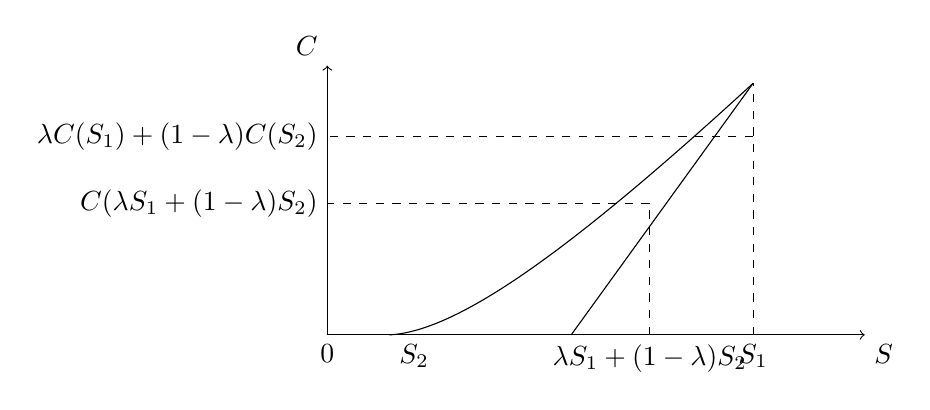
\begin{tikzpicture}[x=1.05cm,y=0.9cm,baseline=(current bounding box.center)]
  \draw[->] (0,0) -- (6.5,0) node[below right] {$S$};
  \draw[->] (0,0) -- (0,3.8) node[above left] {$C$};
  \draw (0.75,0) .. controls (1.6,0.05) and (3.0,1.25) .. (5.15,3.55);
  \draw (2.95,0) -- (5.15,3.55);
  \draw[dashed] (3.9,0) -- (3.9,1.85);
  \draw[dashed] (3.9,1.85) -- (0,1.85);
  \draw[dashed] (5.15,0) -- (5.15,3.55);
  \draw[dashed] (5.15,2.8) -- (0,2.8);
  \node[below] at (0,0) {$0$};
  \node[below] at (1.05,0) {$S_2$};
  \node[below] at (3.9,0) {$\lambda S_1+(1-\lambda)S_2$};
  \node[below] at (5.15,0) {$S_1$};
  \node[left] at (0,1.85) {$C(\lambda S_1+(1-\lambda)S_2)$};
  \node[left] at (0,2.8) {$\lambda C(S_1)+(1-\lambda)C(S_2)$};
\end{tikzpicture}
\caption{Payoff of a European call option}
\label{fig:zhou-figure-6-1}
\end{figure}

If the option is exercised at time $t$, the payoff at $t$ is $C(S_t-K)$. If it is not exercised
until maturity, the discounted expected payoff (to $t$) is $\tilde E[e^{-r\tau}C(S_T)]$ under
risk-neutral measure. Under risk-neutral probabilities, we also have $\tilde E[S_T]=S_te^{r\tau}$.

So $\tilde E[e^{-r\tau}C(S_T)]=e^{-r\tau}\tilde E[C(S_T)]\geq e^{-r\tau}C(\tilde E[S_T])
=e^{-r\tau}C(e^{r\tau}S_t)$, where the inequality is from Jensen's inequality.

Let $S=e^{r\tau}S_t$ and $\lambda=e^{-r\tau}$, we have
$C(\lambda S)=C(S_t)\leq e^{-r\tau}C(e^{r\tau}S_t)\leq e^{-r\tau}\tilde E[C(S_T)]$.

Since the discounted payoff $e^{-r\tau}\tilde E[C(S_T)]$ is no less than $C(S_t)$ for any
$t\leq T$ under the risk neutral measure, it is never optimal to exercise the option before
expiration.

I should point out that the payoff of a put is also a convex function of the stock price.
But it is often optimal to exercise an American put on a non-dividend paying stock. The
difference is that $P(0)=K$, so it does not have the property that $P(\lambda S)\leq\lambda P(S)$.
In fact, $P(\lambda S)\geq\lambda P(S)$. So the argument for American calls does not apply
to American puts.

Similar analysis can also show that early exercise of an American call option for
dividend-paying stocks is never optimal except possibly for the time right before an
ex-dividend date.

\emph{B.} A European put option on a non-dividend paying stock with strike price \$80 is
currently priced at \$8 and a put option on the same stock with strike price \$90 is priced
at \$9. Is there an arbitrage opportunity existing in these two options?
